\section{Date: 2026-11-22}
\noindent \textbf{Series ID: A262RL1Q225SBEA} 

\noindent This series is titled Real Consumption of Fixed Capital and has a frequency of Quarterly. The units are Percent Change from Preceding Period and the seasonal adjustment is Seasonally Adjusted Annual Rate.The observation start date is 1947-04-01 and the observation end date is 2026-07-01.The popularity of this series is 1. \\ 

\noindent \textbf{Series ID: BNEMFT01KRQ460S} 

\noindent This series is titled Business Tendency Surveys for Non-Manufacturing: Employment: Future Tendency: National Indicator for the Republic of Korea (DISCONTINUED) and has a frequency of Quarterly. The units are Net Percent and the seasonal adjustment is Seasonally Adjusted.The observation start date is 1993-01-01 and the observation end date is 2003-01-01.The popularity of this series is 1. \\ 

\subsection{Raw Regression}
\noindent Regresses the two series against each other directly. A significant result here can come just as easily from both series sharing a long-run trend as from any real relationship.

\begin{center}
\begin{tabular}{lclc}
\toprule
\textbf{Dep. Variable:}               & value\_fred\_BNEMFT01KRQ460S & \textbf{  R-squared:         } &     0.099   \\
\textbf{Model:}                       &             OLS              & \textbf{  Adj. R-squared:    } &     0.076   \\
\textbf{Method:}                      &        Least Squares         & \textbf{  F-statistic:       } &     4.280   \\
\textbf{Date:}                        &       Sun, 22 Nov 2026       & \textbf{  Prob (F-statistic):} &   0.0452    \\
\textbf{Time:}                        &           18:45:52           & \textbf{  Log-Likelihood:    } &   -139.74   \\
\textbf{No. Observations:}            &                41            & \textbf{  AIC:               } &     283.5   \\
\textbf{Df Residuals:}                &                39            & \textbf{  BIC:               } &     286.9   \\
\textbf{Df Model:}                    &                 1            & \textbf{                     } &             \\
\textbf{Covariance Type:}             &          nonrobust           & \textbf{                     } &             \\
\bottomrule
\end{tabular}
\begin{tabular}{lcccccc}
                                      & \textbf{coef} & \textbf{std err} & \textbf{t} & \textbf{P$> |$t$|$} & \textbf{[0.025} & \textbf{0.975]}  \\
\midrule
\textbf{const}                        &     -13.1519  &        2.509     &    -5.242  &         0.000        &      -18.227    &       -8.077     \\
\textbf{value\_fred\_A262RL1Q225SBEA} &       0.9965  &        0.482     &     2.069  &         0.045        &        0.022    &        1.971     \\
\bottomrule
\end{tabular}
\begin{tabular}{lclc}
\textbf{Omnibus:}       &  5.178 & \textbf{  Durbin-Watson:     } &    0.537  \\
\textbf{Prob(Omnibus):} &  0.075 & \textbf{  Jarque-Bera (JB):  } &    4.301  \\
\textbf{Skew:}          &  0.787 & \textbf{  Prob(JB):          } &    0.116  \\
\textbf{Kurtosis:}      &  3.194 & \textbf{  Cond. No.          } &     11.5  \\
\bottomrule
\end{tabular}
%\caption{OLS Regression Results}
\end{center}

Notes: \newline
 [1] Standard Errors assume that the covariance matrix of the errors is correctly specified.

\begin{figure}
\centering
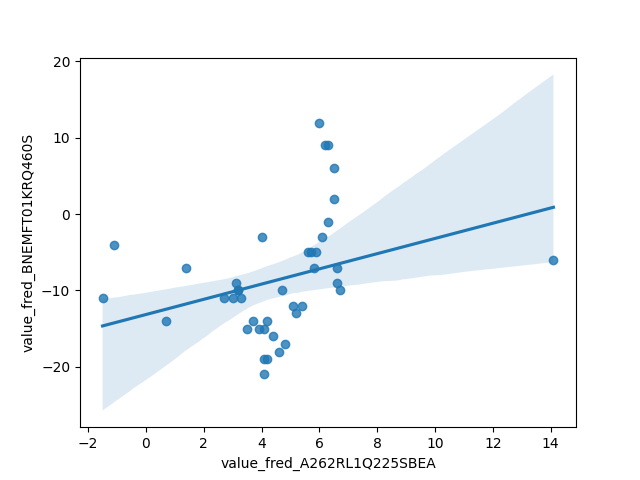
\includegraphics[scale = 0.9]{plots/plot_2026-11-22.png}
\caption{Raw Regression Plot for 2026-11-22}
\end{figure}
\newpage
\subsection{Detrended Regression}
\noindent Regresses the residuals of each series after removing its own linear time trend, so a shared trend can no longer drive the result on its own. A relationship that stays significant here is better evidence of a genuine link between the two series.

\begin{center}
\begin{tabular}{lclc}
\toprule
\textbf{Dep. Variable:}                          & value\_fred\_BNEMFT01KRQ460S\_detrended & \textbf{  R-squared:         } &     0.088   \\
\textbf{Model:}                                  &                   OLS                   & \textbf{  Adj. R-squared:    } &     0.065   \\
\textbf{Method:}                                 &              Least Squares              & \textbf{  F-statistic:       } &     3.776   \\
\textbf{Date:}                                   &             Sun, 22 Nov 2026            & \textbf{  Prob (F-statistic):} &   0.0592    \\
\textbf{Time:}                                   &                 18:45:52                & \textbf{  Log-Likelihood:    } &   -136.67   \\
\textbf{No. Observations:}                       &                      41                 & \textbf{  AIC:               } &     277.3   \\
\textbf{Df Residuals:}                           &                      39                 & \textbf{  BIC:               } &     280.8   \\
\textbf{Df Model:}                               &                       1                 & \textbf{                     } &             \\
\textbf{Covariance Type:}                        &                nonrobust                & \textbf{                     } &             \\
\bottomrule
\end{tabular}
\begin{tabular}{lcccccc}
                                                 & \textbf{coef} & \textbf{std err} & \textbf{t} & \textbf{P$> |$t$|$} & \textbf{[0.025} & \textbf{0.975]}  \\
\midrule
\textbf{const}                                   &   -1.557e-12  &        1.086     & -1.43e-12  &         1.000        &       -2.197    &        2.197     \\
\textbf{value\_fred\_A262RL1Q225SBEA\_detrended} &       0.8735  &        0.450     &     1.943  &         0.059        &       -0.036    &        1.783     \\
\bottomrule
\end{tabular}
\begin{tabular}{lclc}
\textbf{Omnibus:}       &  8.006 & \textbf{  Durbin-Watson:     } &    0.572  \\
\textbf{Prob(Omnibus):} &  0.018 & \textbf{  Jarque-Bera (JB):  } &    6.945  \\
\textbf{Skew:}          &  0.960 & \textbf{  Prob(JB):          } &   0.0310  \\
\textbf{Kurtosis:}      &  3.619 & \textbf{  Cond. No.          } &     2.42  \\
\bottomrule
\end{tabular}
%\caption{OLS Regression Results}
\end{center}

Notes: \newline
 [1] Standard Errors assume that the covariance matrix of the errors is correctly specified.

\begin{figure}
\centering
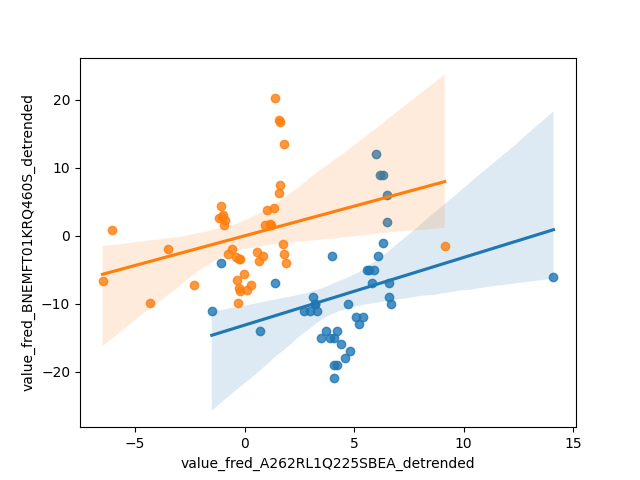
\includegraphics[scale = 0.9]{plots/plot_2026-11-22_detrended.png}
\caption{Detrended Regression Plot for 2026-11-22}
\end{figure}
\newpage
